\chapter{Summary}
This thesis focuses on power grid and, in particular, on the problems introduced by the distributed energy resources devices. These devices generate electricity from natural resources (solar, wind, ...) that allows to satisfy the energy demand directly in place (photovoltaic panels on a rooftop) or close to where it is consumed (photovoltaic farms, ...). This new energy production system goes against the traditional power networks structure, where the electricity is produced in big power plants and transmitted to where it is requested, for a more decentralised approach, where almost everyone can be an active part of the network producing electricity. This decentralised system introduces some complications in the networks. Indeed, the energy that flows from many sources generates some possible voltage problems on the different devices of the network, like for example line, buses, and other elements. In particular, the problems introduced by the distributed energy devices are over voltage problems: that is, when the voltage is above a standard voltage value.\\

% This thesis investigates on forecasting the network's over voltage situations and on controlling the network's devices to avoid these problems.

\section{Aim of the thesis}
The aim of this thesis is to exploit data-driven approaches to forecast the future nodes' voltage based on historical measurements in a medium-voltage distribution system using machine learning techniques, in particular deep artificial neural networks. The objectives of this thesis are to:
\begin{itemize}
    \item Build a dataset of time series that is used to train the machine learning models. A real medium-voltage network from the Pandapower python library is used. This network is fit with time series taken from the Simbench database, a database generated by the measurements of real loads and generators from Germany. 
    \item Predict the voltage fluctuation problems in the network under a supervised learning framework. The three artificial neural networks used are: a multi layer perceptron, a convolutional neural network and a recurrent neural network. Three combinations of network information are tested, and some techniques for unbalanced datasets are tested as well. \\
    Different combinations are used since the network operator can have access to a limited amount of data, so the performances for each combination are reported.
    \item Control the active and reactive power of the network's generators using reinforcement leaning framework. The model used is a deep deterministic policy gradient algorithm that allows to work with continuos state and action space.
\end{itemize}
Predicting the contingency problems and controlling the network's devices would allow reducing possible consequences related to voltage issues, like for example over voltages problems. 

\section{MV Oberrhein network}
The thesis is developed in Pandapower, an open-source and popular Python library that makes it easy to work with power networks.\\
Among all the power networks available in the Pandapower library, the one used for these experiments is the MV Oberrhein network. MV Oberrhein is a real distribution located at Upper Rhine (in German:  Oberrhein),  Germany. 

\begin{figure}[H] 
\centering
\subfloat
    {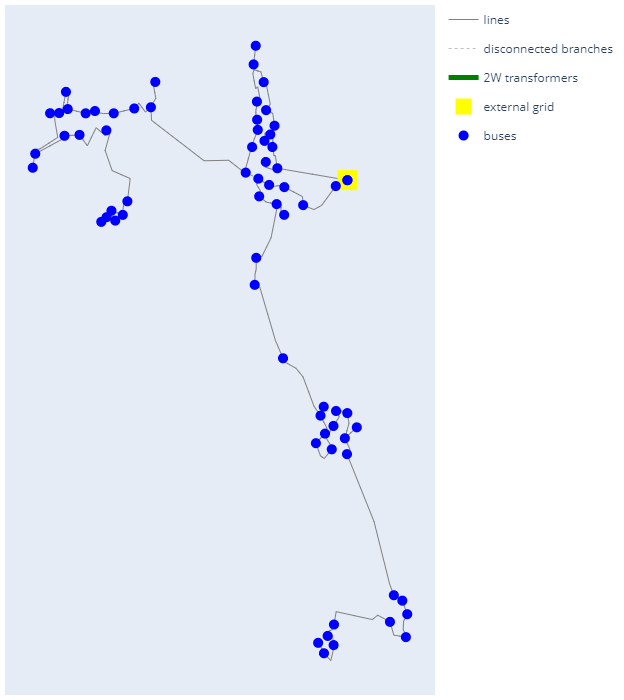
\includegraphics[width=0.4\linewidth]
    {images/MVOberr/MVOberr_half1.png}}
\caption[MV Oberrhein network division]{MV Oberrhein network}
\label{fig:MVObbB}
% \label{fig:MVoberdiv}
\end{figure}

\noindent The network used in this thesis is the one showed in figure \ref{fig:MVObbB}. The network consists of: one external grid, one transformer, 70 buses, 61 loads and 60 generators.

\section{Simbench database}
The time series used is taken from the Simbench database. This database refers to some real distribution networks in Germany of the year 2016. SimBench includes multiple time series for one year with 15 min resolution for loads, generators and storage units.\\

Power utilities commonly use generic load profiles to group commercial customers with similar load shapes into categories or standard load profiles.

\section{Time series selection}
Some time series from the Simbench database are taken to adapt to the number of loads and distributed energy resources devices of the MV Oberrhein network in consideration. \\

In this case, the profile's types for loads and distributed energy resources devices are chosen, such that every profile type is present, to have a network as close as possible to a real network. \\

\begin{figure}[H]
\centering
    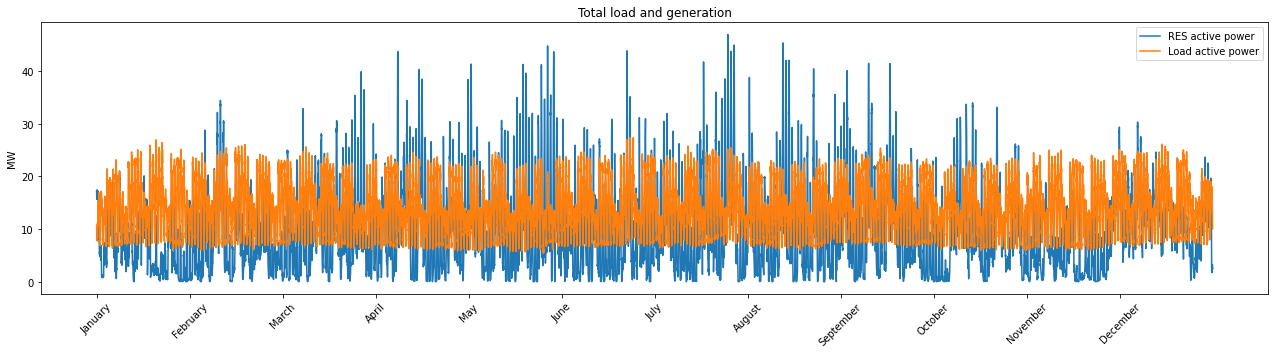
\includegraphics[width=1\linewidth]{images/MVOberr/Load&Gens.png}
\caption[Consumed and generated energy]{Sum of load energy consumption and energy generation over the considered year.}
% \label{fig:gym_anm_net}
\end{figure}

The load consumption values are as a typical MV network, while the generation is higher. This case can represent a future power network when the number and the performance of distributed energy resources devices increase, so to have a generation of power higher than the demand; especially during the summer period when the consumption is lower and the generation is higher.\\
Such situations are critical for a network since the surplus energy increases the voltages at the buses that may experience voltage problems.\\


In this thesis, the network situation, in a given time step $t$, is considered critical if the voltage of at least one of the buses is out of the boundaries $V_t < v^{\text{min}}$ (under voltage) or $V_t > v^{\text{max}}$ (over voltage), where $v^{\text{min}}$ is the minimum acceptable voltage, $0.95$ p.u. (per unit), and $v^{\text{max}}$ is the maximum one, $1.05$ p.u.\\
\begin{figure}[H]
\centering
    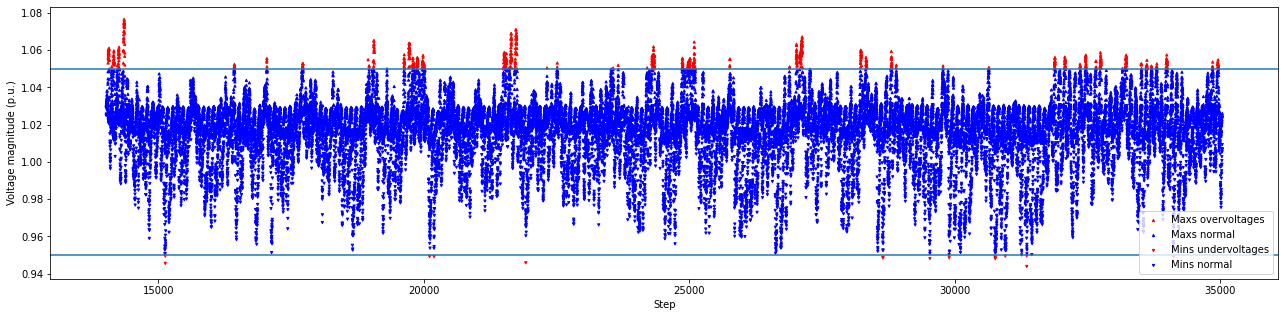
\includegraphics[width=1\linewidth]{images/MVOberr/CritialSituationsBefore.png}
\caption[Network's critical situations]{Network's over and under voltage critical situations. The two horizontal lines correspond to $v^{\text{max}}$ and $v^{\text{min}}$.}
\label{fig:ctb}
\end{figure}

In figure \ref{fig:ctb}, it is possible to see that the number of over voltages situations is low compared to the normal situations. It is possible to see that there are also few under voltage situations.



\section{Problem statement}
\label{sec:4ps}
This thesis focuses on active network management (ANM) and the problem faced by a distribution system operator (\gsl{DSO}) to maintain the network within its operational limits. In particular, the system operator evaluates whether at a given moment there will be a voltage problem. In this way, the \gls{DSO} can proceed with some actions, like applying curtailment to generator devices or control their reactive power, to maintain the voltage inside a safe range.\\

For this problem, we assume that the \gls{DSO} knows the following information:
\begin{itemize}
    \item The network topology: the number of buses, loads and generators, the lines' length and impedance.
    
    \item The active and reactive power of some loads at each time step.
    
    \item The type of \gsl{DER} device connected to each bus.
\end{itemize}

This data is used to calculate the power flow of the network and obtain more information like the voltage magnitude at each bus, lines' loading and other values.\\

A power network can be represented as a direct graph $\mathsf{G}(\mathcal{N},\mathcal{E})$, where \gls{N} is a set of nodes, also called buses ($\mathcal{B}$), in the network; \gls{E} $\subseteq \mathcal{N} \times \mathcal{N}$ is the set of directed edges linking two buses together, also called lines. The notation \gls{e} $\in \mathcal{E}$ refers to the directed edge with sending bus $i$ and receiving bus $j$. Each bus might be connected to several devices, which may inject or withdraw power from the grid. The set of all devices is denoted by \gls{D} that can be either loads \gls{L} or generators \gls{G}. Let's also define \gls{T} as the set of transformers. \\

% https://arxiv.org/ftp/arxiv/papers/2102/2102.05657.pdf
The \gls{DSO} considers the behaviour of the network over a set of discrete time steps $t \in \{1,2,...,T-1,T\}$ of length $\Delta t$, with, $T \in \mathbb{N}$, the last time step of the time series’ horizon. A time step is considered as a snapshot of the system at one particular point in time. \\ 

The \gls{DSO} can have access to some information, let's define $\textbf{I}$ as the information domain. This information can be divided in static information like the network topology, and the observation $\mathbf{O_t}$ collected at every time step $t$ like the loads and generators' active and reactive power and the buses' voltage magnitude and lines' loading. The information at time step $I_t$ can be defined as:
\begin{align*}
    \mathbf{I_t} & \in \mathbf{I}, \text{with} \, t \in \{1,2,...,T-1,T\} \\
    \mathbf{I_t} & = [\mathbf{{static}} \, \mathbf{{information}}, \mathbf{O_t}]
\end{align*}
\noindent In general power networks are not static, since the operators can modify their topology, for example changing the connections due to some incidents on the lines. In this thesis, the network topology is considered as static, so that no changes are applied on the network during the whole time series' horizon.\\

\noindent An instance of the observation $\mathbf{O_t}$ can be:
\begin{equation*}
    \mathbf{O_t} =  [
            \mathbf{\mathcal{L}^p_{t}}, 
            \mathbf{\mathcal{L}^q_{t}}, 
            \mathbf{\mathcal{G}^p_{t}},
            \dots ]
\end{equation*}
\noindent where $\mathbf{\mathcal{L}^p_{t}}$ and $\mathbf{\mathcal{L}^q_{t}}$ are active and reactive power of loads $\mathcal{L}$ at timestamp $t$; $\mathbf{\mathcal{G}^p_{t}}$ is the active power of the generators $\mathcal{G}$ at time $t$; some other variables can be included in the observation $\mathbf{O_t}$ for example the buses' voltage magnitudes or the loading percentage of each line etc.\\

For the forecasting part, the operator predicts if the system, at some given $t+n$ future time steps, will be in a critical condition. The network is considered in a critical condition if any of its elements is in an unsafe situation, for example an over voltage condition. Let define $\textbf{C}$ as the list of critical situations and $C_t$ the critical situation at time step $t$, with $C_t \in \{0,1\}$.  \\
For predicting whether the system will be in a critical situation or not, the \gls{DSO} considers the history of the system only for $h$ preceding steps, with $h \in \mathbb{N}^+$. \\

\section{Solving methodology}
\subsection{Forecasting}
The goal of this section is to train a classifier that can forecast whether in the future there will be some over voltage problems.\\

As a supervised task, the time series are separated in training and testing dataset; in particular, the data is divided in windows of length, $h$ for the inputs $\textbf{x}$ and length $n$ for the outputs $\textbf{y}$. \\

There are many ways and combinations of how to choose the information used for the input $\textbf{x}$s. In this thesis, three combinations are tested:

\begin{enumerate}[label=\textbf{\roman*)}]
    \item \label{onlyV} Considering only the voltage information at each bus.
    \begin{equation}
      \begin{aligned}
        \textbf{x}  &= [\mathbf{V_{t-h+1}}, \mathbf{V_{t-h+2}}, \dots, \mathbf{V_{t-1}}, \mathbf{V_{t}}]
      \end{aligned}
    \end{equation}
    \noindent where $\mathbf{V_t}$ is the voltage level \gls{V} of every bus $\mathcal{B}$ at timestamp $t$.
    
    \item \label{LpqandGp} Considering active and reactive power of loads and active power of generators.
    \begin{equation}
      \begin{aligned}
        \textbf{x}  &= [
            \mathbf{\mathcal{L}^p_{t-h+1}}, \mathbf{\mathcal{L}^q_{t-h+1}}, \mathbf{\mathcal{G}^p_{t-h+1}},
            \dots,
            \mathbf{\mathcal{L}^p_{t}}, 
            \mathbf{\mathcal{L}^q_{t}}, 
            \mathbf{\mathcal{G}^p_{t}}]
      \end{aligned}
    \end{equation}
    \noindent where $\mathbf{\mathcal{L}^p_{t}}$ and $\mathbf{\mathcal{L}^q_{t}}$ are, respectively, the active and reactive power of all loads \gls{L} at timestamp $t$ and $\mathbf{\mathcal{G}^p_{t}}$ is the active power of each generator \gls{G} at timestamp $t$.
    
    \item \label{GpandTpq} Considering active power of generators and the active and reactive power at the transformer on the HV/MV substation.
    \begin{equation}
      \begin{aligned}
        \textbf{x}  &= [
            \mathbf{\mathcal{G}^p_{t-h+1}}
            \mathcal{T}^p_{t-h+1},
            \mathcal{T}^q_{t-h+1}, 
            \dots,
            \mathbf{\mathcal{G}^p_{t}}, 
            \mathcal{T}^p_{t}, 
            \mathcal{T}^q_{t}]
      \end{aligned}
    \end{equation}
    \noindent where $\mathcal{T}^p_{t}$ and $\mathcal{T}^q_{t}$ are, respectively, the active and reactive power of the transformer at timestamp $t$.
    
    \item \label{case4} Since the considered dataset is unbalanced, some techniques usually used when dealing with these kinds of datasets are employed. The techniques are: over and under sampling and set weights for each class.\\
    These techniques are tested on the best and worst performing models of all the aforementioned combinations.
    % \ref{onlyV}, \ref{LpqandGp}, \ref{GpandTpq}
\end{enumerate}
\noindent Different combinations are considered because it is interesting to check how the model performs with different kinds of data; moreover, the information a \gls{DSO} can have access to can be limited, so some cases are more realistic than others. In particular, \gls{DSO} usually has access to only a limited amount of data: for small loads (households, ...) the active and reactive powers are not available at every instant (they are only after some period of time, after the bill is issued), in general the more a device is close to the transformer the more information a \gld{DSO} has access to, so the combination \ref{GpandTpq} would be the most appropriate for a MV network.\\


\noindent For the labels, $\textbf{y}$ can be defined as: 
\begin{equation} \label{eq:labels}
    \begin{aligned}
        \textbf{y} = [C_{t+1},C_{t+2}, \dots, C_{t+n-1},C_{t+n}]
    \end{aligned}
\end{equation}
\noindent where $C_t$ is the condition of the system at timestamp $t$, with $C_t=1$ if the network is in a critical situation or $C_t=0$ if it is in a normal situation and $n$ is the number of future time steps considered, with $n \in \mathbb{N}^+$. \\

For what concerns $h$, the number of history step considered and $n$, the number of future steps to forecast, these are not hyperparameter to be optimised, but are values that depend on the problem and the task that a \gls{DSO} is trying to solve. In particular, choosing a value of $h$ depends on the amount of data the \gls{DSO} can access to, the computation cost and the time to get an answer; while $n$, depends on the kind of forecasting the \gls{DSO} wants to apply, either short planning, medium-term planning or long-term planning.\\

The couples $\{\textbf{x},\textbf{y}\}$ are divided in training, validation and test set, with the following ratios: $0.7$, $0.2$, $0.1$.\\
For the forecasting part, only over voltages are considered. These are the critical states' distribution in training, validation and test sets.
\begin{algorithm}[H]
    \State Number of over voltage situations: 1229, over 35040 time steps, ratio: 3.5\% \\
    
    \State Number of over voltage situations in Training set: 835, ratio: 3.4\%\\
    \State Number of over voltage situations in Validation set: 211, ratio: 3.0\%\\
    \State Number of over voltage situations in Testing set: 183, ratio: 5.2\%
\end{algorithm}

Three different \glspl{ANN} are tested: MLP, CNN, RNN.\\

The trained model predicts the critical condition of the system at some future time steps $n$. Let's define $\hat{\textbf{y}} = \hat{\textbf{C}}$ as the forecasted values of the system given the information $\textbf{x} \in \textbf{I}$. 
% A single instance $\hat{C}_{t+i}$ ($\hat{C}_{t+i} \in \{0,1\}$) states if the system is critical ($\hat{C}_{t+i}=1$) or not ($\hat{C}_{t+i}=0$), with $i \in \{1,2,\dots,n-1,n\}$ and $n \in \mathbb{N}^+$.\\

The main goal of the model is predicting the future values such that the actual critical values $\textbf{C}$ and forecasted values $\hat{\textbf{C}}$ are as close as possible.


\subsection{Active control}
The goal of this section is to train an agent that can take some action to solve the voltage problems.\\

The agent is trained within a reinforcement learning context. Let's define the main \gls{RL} elements:
\begin{itemize}
    \item \emph{Environment}. The environment is the entire grid, so the MV Oberrhein network.
    
    \item \emph{State}. The state is the information the agent can have access to. In this case, active and reactive power of loads and active power of generators at time step $t$. \\
    \[
        \mathbf{s_t} = [\mathbf{\mathcal{L}^p_{t}},                             \mathbf{\mathcal{L}^q_{t}},                             \mathbf{\mathcal{G}^p_{t}}]
    \]
    \noindent So the state is a list of continuos variables of size 182 ($|\mathcal{L}|+|\mathcal{L}|+|\mathcal{G}| = 61 + 61 + 60$).

    \item \emph{Action}. The agent can control active and reactive power of the generators, in particular:
    \[
        \mathbf{a_t} = [\mathbf{a^p_t}, \mathbf{a^q_t}]
    \]
    with $\mathbf{a^p_t}$ an array with the active power reducing factors at time step $t$ ($a^p_{t,i} \in [0,1]$ and $i \in {1, ..., |\mathcal{G}|}$) and $\mathbf{a^q_t}$ an array with reactive powers values ($a^q_{t,i} \in [-0.25,0.25]$). So the state is a list of continuos variables of size 120 ($2 \cdot |\mathcal{G}|$).\\
    
    These values are used to change active and reactive power of the generators at the time step $t+1$.\\
    $\mathbf{a^p_t}$ represents the proportion of the quantity of energy curtailment decided by the agent. In formula:
    \[
        \mathbf{final\_power_{t+1}} = \mathbf{initial\_power_{t+1}} \cdot (\mathbf{1}-\mathbf{a^p_t})
    \]
    \noindent with $\mathbf{initial\_power_{t+1}}$ the initial power the generator was about to output at time step ${t+1}$ (same as $\mathbf{\mathcal{G}^p_{t+1}}$. The notation $\mathbf{initial\_power}$ is used for a clearer understanding of what happens before and after the agent action); $\mathbf{final\_power_{t+1}}$ the curtailed power, actual power output.\\
    
    For the reactive power, $\mathbf{a^q_t}$ represents the quantity of reactive power absorbed or injected in the network by each generator. 
    
    
    \item \label{4:rewfunc} \emph{Reward function}. The reward function consists of four terms:
    \begin{itemize}
        \item A reward regarding the active power. The agent is punished to choose too high values of active power curtailment, the higher the curtailment, the higher the punishment.
        \[
            reward\_p_t = -\sum_{i=0}^{|\mathcal{G}|}a^p_{t,i}
        \]
        
        \item A reward for the reactive power. The agent is punished proportionally to the change in the values of reactive power. 
        \[
            reward\_q_t = -\sum_{i=0}^{\mathcal{G}} |a^q_{t,i}|
        \]
        \noindent the $|\cdot|$ is needed, since $\mathbf{a^q_t}$ may contain both positive and negative values.
        
        \item A reward regarding voltage violation. The agent is punished if the voltage magnitude of the buses is away from 1 p.u. The punishment value is chosen with the following a punishment function $f$:
        \begin{figure}[H]
        \centering
            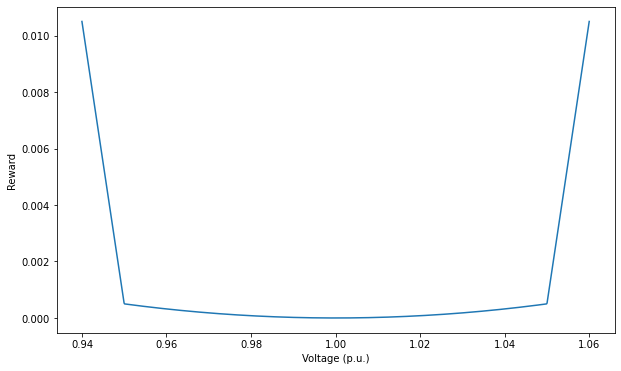
\includegraphics[width=.4\linewidth]{images/MVOberr/RL/volatge_violation_function.png}
            \caption[Voltage violation function]{Shape of the voltage violation function centred in 1 p.u.}
        \end{figure}
        \noindent The idea is to punish the agent by a low value when the voltage bus is in the range [0.95,1.05] and to punish it more when the voltage bus is more far away from 1 p.u.
        \[
            reward\_vv_t = -\sum_{i=0}^{|\mathcal{B}|} f(V^{i}_{t+1})
        \]
        
        \item A reward for the critical situation solved. The agent is given a positive or negative reward whether it was able to solve the critical situation or not. In particular:\\
        \[
            reward\_cs_t =  C_{t+1} - 4 \cdot network\_status_{t+1}
        \]
        with $C_{t+1}$ the critical status of the network as stated in the forecasting section (expression \ref{eq:labels}) at time step $t+1$, and $network\_status_{t+1}$ a boolean value stating if the system at time step $t+1$, after the agent action and the \gls{PF} calculation, is critical or not.\\
        The main idea is to make the agent understand if the chosen action was helpful and solved the critical situation of the network. In particular, there are four possible cases:\\
        
        \begin{itemize}[leftmargin=2cm]\label{im:cases}
            \item[case 1)] 0 - 0: no critical situation before and after the agent's action (good, $0$ reward).
            \item[case 2)] 0 - 1: no critical situation before, but it was introduced by the agent's action (the worst case, $-4$ reward).
            \item[case 3)] 1 - 0: critical situation before and it was solved by the agent's action (the best case, $+1$ reward).
            \item[case 4)] 1 - 1: critical situation before and after the agent's action (not good, $-3$ reward).
        \end{itemize}
        
    \end{itemize}
    The total reward is given by the algebraic sum of all the previous terms multiplied by a scaling factor:
    \begin{equation} \label{eq:rew}
      \begin{aligned}
            reward_t = &\hphantom{..,,} 
                          \alpha_p \cdot reward\_p_t + \\
                       &+ \alpha_q \cdot reward\_q_t + \\
                       &+ \beta \cdot reward\_vv_t + \\
                       &+ \gamma \cdot reward\_cs_t
      \end{aligned}
    \end{equation}
    with $\alpha_p=4$, $\alpha_q=2$, $\beta=100$ and $\gamma=20$. These values are chosen to balance the rewards get by the agent.\\
    With such articulate reward expressed in \ref{eq:rew}, the agent's goal is to reduce the number of over voltage situation without introducing new under voltage situations.
    
    \item \emph{Agent}. The agent model chosen is the \gls{DDPG} algorithm. This algorithm can handle continuous state and action spaces, so it is suitable for this task.
    
\end{itemize}

The agent is trained using $40\%$, $14016$ time steps, of the data and tested on the remaining $60\%$, $21024$ time steps. The training is repeated for $4$ time for a total of $56064$ time steps.\\

% \begin{algorithm}[H]
%   \caption{Pseudo-algorithm for the control of the network's devices}
%   \begin{algorithmic}
%     \STATE Initialize the network
%     \STATE Extract time series for each time step from Simbench database
%     \STATE Calculate \gls{PF} for each time step and evaluate when the system is in a critical situation, obtaining $\textbf{C}$
%     \STATE Initialize agent with actor and critic networks: $\phi$, $\theta$, $\phi_{target}$ and $\theta_{target}$ 
%     \FOR{ each episode $p$ } 
%         \FOR{ each time step $t \in \{1,2,\dots,T-2,T-1\}$ }
%             \STATE Get state $\mathbf{s_t}$ from the network
%             \STATE Choose the action $\mathbf{a_t}$ with $\mathbf{a_t}=\phi(\mathbf{s_t})$
%             \STATE Get active power of the generators at time step $t+1$: $\mathbf{initial\_power_{t+1}}$
%             \STATE Apply the action: change active and reactive power of the generators at time step $t+1$ with the $\mathbf{final\_power_{t+1}}$
%             \STATE Calculate the \gls{PF} at the time step $t+1$
%             \STATE Calculate the reward $r_t$, as mentioned in \ref{4:rewfunc}
%             \STATE Check the status of the environment: $d_t$
%             \STATE Get new state $\mathbf{s_{t+1}}$
%             \STATE Store the experience ($\mathbf{s_t}, \mathbf{a_t}, r_t, \mathbf{s_{t+1}}, d_t$)
%             \STATE Train the agent
%         \ENDFOR
%     \ENDFOR
%   \end{algorithmic}
% \end{algorithm}

\section{Results and analysis}
\subsection{Forecast results}
For the forecasting task, some evaluation metrics are used to test the performance of the \gls{ANN}. These metrics are: accuracy, recall, precision and F1-score. \\
During training, the F1-score on the validation set of the model is monitored, and the best one is saved. The score reported in the following tables, are obtained testing the model on the test set, with the most performing saved model. \\

In this thesis, three values of $h$ are used: 2, 4 and 16 corresponding to have the past information of the system of 30 minutes, 1 hour and 4 hours. For the $n$, only one value is used: 1, corresponding to a short planning time of 15 minutes ahead.\\

The three combinations are tested, and the results are reported as average of 5 runs:
% \begin{enumerate}[label=\roman*)]
\begin{itemize}
    \item Results of the first combination \ref{onlyV}:
    
    \begin{table}[H]
    \centering
    \begin{tabular}{|c|l|c|c|c|c|}
    \hline
    \textbf{h} &
      \textbf{Models} &
      \multicolumn{1}{l|}{\textbf{Accuracy}} &
      \multicolumn{1}{l|}{\textbf{Precision}} &
      \multicolumn{1}{l|}{\textbf{Recall}} &
      \multicolumn{1}{l|}{\textbf{F1-score}} \\ \hline
    \multirow{3}{*}{\textbf{2}}  & \textbf{MLP} & 0.979 & 0.786 & 0.833 & 0.804 \\ \cline{2-6} 
                                 & \textbf{CNN} & 0.981 & 0.793 & 0.862 & 0.825 \\ \cline{2-6} 
                                 & \textbf{RNN} & 0.981 & 0.798 & 0.858 & \textbf{0.826} \\ \hline
    \multirow{3}{*}{\textbf{4}}  & \textbf{MLP} & 0.979 & 0.817 & 0.777 & 0.792 \\ \cline{2-6} 
                                 & \textbf{CNN} & 0.980 & 0.795 & 0.851 & 0.820 \\ \cline{2-6} 
                                 & \textbf{RNN} & 0.981 & 0.796 & 0.860 & \textbf{0.827} \\ \hline
    \multirow{3}{*}{\textbf{16}} & \textbf{MLP} & 0.978 & 0.800 & 0.797 & 0.796 \\ \cline{2-6} 
                                 & \textbf{CNN} & 0.798 & 0.798 & 0.822 & 0.810 \\ \cline{2-6} 
                                 & \textbf{RNN} & 0.980 & 0.786 & 0.866 & \textbf{0.823} \\ \hline
    \end{tabular}
    \caption[Models' results using voltage information]{Results using as input the voltage information at each bus.}
    \label{tab:onlyV}
    \end{table}
    This task is the simplest case, since the goal is to predict the future of a particular quantity (voltage) given the past information of the same quantity.\\
    From table \ref{tab:onlyV}, It is possible to see that the \gls{RNN} model performs better than the other models, since usually \gls{RNN} handles better time series data. Moreover, it would be expected that the more data the \glspl{ANN} receive as input (value of h), the higher the score it gets, but for this task, results look like are independent of the value of $h$.
    
    \item Results of the second combination     \ref{LpqandGp}:
    
    \begin{table}[h]
    \centering
    \begin{tabular}{|c|l|c|c|c|c|}
    \hline
    \textbf{h} &
      \textbf{Models} &
      \multicolumn{1}{l|}{\textbf{Accuracy}} &
      \multicolumn{1}{l|}{\textbf{Precision}} &
      \multicolumn{1}{l|}{\textbf{Recall}} &
      \multicolumn{1}{l|}{\textbf{F1-score}} \\ \hline
    \multirow{3}{*}{\textbf{2}}  & \textbf{MLP} & 0.961 & 0.960 & 0.263 & 0.399 \\ \cline{2-6} 
                                 & \textbf{CNN} & 0.969 & 0.948 & 0.429 & 0.570 \\ \cline{2-6} 
                                 & \textbf{RNN} & 0.969 & 0.907 & 0.451 & \textbf{0.591} \\ \hline
    \multirow{3}{*}{\textbf{4}}  & \textbf{MLP} & 0.963 & 0.962 & 0.308 & 0.454 \\ \cline{2-6} 
                                 & \textbf{CNN} & 0.965 & 0.945 & 0.359 & \textbf{0.510} \\ \cline{2-6} 
                                 & \textbf{RNN} & 0.963 & 0.955 & 0.325 & 0.473 \\ \hline
    \multirow{3}{*}{\textbf{16}} & \textbf{MLP} & 0.969 & 0.815 & 0.542 & 0.623 \\ \cline{2-6} 
                                 & \textbf{CNN} & 0.971 & 0.843 & 0.580 & \textbf{0.665} \\ \cline{2-6} 
                                 & \textbf{RNN} & 0.969 & 0.912 & 0.467 & 0.603 \\ \hline
    \end{tabular}
    \caption[Models' results using loads and generators information]{Results using as input the active and reactive power of each load and active power of each generator.}
    % \label{tab:my-table}
    \end{table}
    This combination performs the worst. These results can be explained considering the complexity and non-linearity of the \gls{PF} calculation. So the models are not able to grasp the relationship that maps the loads and generators' information to the buses' voltage. Moreover, the \glspl{ANN} are missing all the information regarding the network, like for example the lines' resistance, impedance etc; essential for the \gls{PF} calculation. Another possible explanation is a large input space.
    
    
    \item Results of the third combination \ref{GpandTpq}:
    
    \begin{table}[h]
    \centering
    \begin{tabular}{|c|l|c|c|c|c|}
    \hline
    \textbf{h} &
      \textbf{Models} &
      \multicolumn{1}{l|}{\textbf{Accuracy}} &
      \multicolumn{1}{l|}{\textbf{Precision}} &
      \multicolumn{1}{l|}{\textbf{Recall}} &
      \multicolumn{1}{l|}{\textbf{F1-score}} \\ \hline
    \multirow{3}{*}{\textbf{2}}  & \textbf{MLP} & 0.974 & 0.727 & 0.837 & 0.774          \\ \cline{2-6} 
                                 & \textbf{CNN} & 0.972 & 0.683 & 0.897 & 0.773          \\ \cline{2-6} 
                                 & \textbf{RNN} & 0.974 & 0.692 & 0.915 & \textbf{0.788} \\ \hline
    \multirow{3}{*}{\textbf{4}}  & \textbf{MLP} & 0.971 & 0.683 & 0.893 & \textbf{0.769} \\ \cline{2-6} 
                                 & \textbf{CNN} & 0.966 & 0.619 & 0.950 & 0.748          \\ \cline{2-6} 
                                 & \textbf{RNN} & 0.970 & 0.669 & 0.910 & 0.764          \\ \hline
    \multirow{3}{*}{\textbf{16}} & \textbf{MLP} & 0.964 & 0.628 & 0.887 & 0.728          \\ \cline{2-6} 
                                 & \textbf{CNN} & 0.970 & 0.679 & 0.873 & 0.757          \\ \cline{2-6} 
                                 & \textbf{RNN} & 0.973 & 0.703 & 0.899 & \textbf{0.782} \\ \hline
    \end{tabular}
    \caption[Models' results using generators and the external grid information]{Results using as input the active each generator and the active and reactive power of the external grid's transformer.}
    % \label{tab:my-table}
    \end{table}
    This case is the more realistic one, since a \gls{DSO} has always the information at the transform on the external grid and the active power of the generators as well.\\
    The score is lower than combination \ref{onlyV} but better than combination \ref{LpqandGp}.\\
    
    \item Testing some techniques for unbalanced datasets \ref{case4}:
    
    \begin{table}[h]
    \centering
    \resizebox{0.9\textwidth}{!}{%
    \begin{tabular}{|c|l|l|c|c|c|c|}
    \hline
    \textbf{Method} &
      \textbf{h} &
      \textbf{Model} &
      \multicolumn{1}{l|}{\textbf{Accuracy}} &
      \multicolumn{1}{l|}{\textbf{Precision}} &
      \multicolumn{1}{l|}{\textbf{Recall}} &
      \multicolumn{1}{l|}{\textbf{F1-score}} \\ \hline
    \textbf{\begin{tabular}[c]{@{}c@{}}Reference\\ \textcolor{white}{.}\end{tabular}} &
      \multirow{4}{*}{2} &
      \multirow{4}{*}{MLP} &
      \begin{tabular}[c]{@{}c@{}}0.960\\ (0.005)\end{tabular} &
      \begin{tabular}[c]{@{}c@{}}0.959\\ (0.021)\end{tabular} &
      \begin{tabular}[c]{@{}c@{}}0.263\\ (0.107)\end{tabular} &
      \begin{tabular}[c]{@{}c@{}}0.399\\ (0.147)\end{tabular} \\ \cline{1-1} \cline{4-7} 
    \textbf{\begin{tabular}[c]{@{}c@{}}Over\\ sampling\end{tabular}} &
       &
       &
      \begin{tabular}[c]{@{}c@{}}0.973\\ (0.005)\end{tabular} &
      \begin{tabular}[c]{@{}c@{}}0.912\\ (0.046)\end{tabular} &
      \begin{tabular}[c]{@{}c@{}}0.555\\ (0.149)\end{tabular} &
      \begin{tabular}[c]{@{}c@{}}0.673\\ (0.106)\end{tabular} \\ \cline{1-1} \cline{4-7} 
    \textbf{\begin{tabular}[c]{@{}c@{}}Under\\ sampling\end{tabular}} &
       &
       &
      \begin{tabular}[c]{@{}c@{}}0.953\\ (0.003)\end{tabular} &
      \begin{tabular}[c]{@{}c@{}}0.625\\ (0.093)\end{tabular} &
      \begin{tabular}[c]{@{}c@{}}0.422\\ (0.307)\end{tabular} &
      \begin{tabular}[c]{@{}c@{}}0.420\\ (0.215)\end{tabular} \\ \cline{1-1} \cline{4-7} 
    \textbf{\begin{tabular}[c]{@{}c@{}}Classes\\ weights\end{tabular}} &
       &
       &
      \begin{tabular}[c]{@{}c@{}}0.971\\ (0.003)\end{tabular} &
      \begin{tabular}[c]{@{}c@{}}0.854\\ (0.083)\end{tabular} &
      \begin{tabular}[c]{@{}c@{}}0.5710\\ (0.134)\end{tabular} &
      \begin{tabular}[c]{@{}c@{}}0.667\\ (0.073)\end{tabular} \\ \hline
    \end{tabular}%
    }
    \caption[Worst model's results testing some techniques for unbalanced datasets]{Results for the worst performing model using as input the active of each generator and the active and reactive power of the external grid's transformer. The value between brackets is the standard deviation.}
    % \label{tab:m}
    \end{table}
    \noindent It is possible to see that the score increases in all the cases, with the highest improvement with the over sampling method. While the lowest improvement is obtained with the under sampling techniques. A possible explanation is that during this operation, it may remove useful data that can be essential for the models.
    
    \begin{table}[h]
    \centering
    \resizebox{0.9\textwidth}{!}
    {%
    \begin{tabular}{|c|l|l|c|c|c|c|}
    \hline
    \textbf{Method} &
      \textbf{h} &
      \textbf{Model} &
      \multicolumn{1}{l|}{\textbf{Accuracy}} &
      \multicolumn{1}{l|}{\textbf{Precision}} &
      \multicolumn{1}{l|}{\textbf{Recall}} &
      \multicolumn{1}{l|}{\textbf{F1-score}} \\ \hline
    \textbf{\begin{tabular}[c]{@{}c@{}}Reference\\ \textcolor{white}{.}\end{tabular}} &
      \multirow{4}{*}{2} &
      \multirow{4}{*}{RNN} &
      \begin{tabular}[c]{@{}c@{}}0.981\\ (0.0004)\end{tabular} &
      \begin{tabular}[c]{@{}c@{}}0.798\\ (0.014)\end{tabular} &
      \begin{tabular}[c]{@{}c@{}}0.858\\ (0.013)\end{tabular} &
      \begin{tabular}[c]{@{}c@{}}0.826\\ (0.001)\end{tabular} \\ \cline{1-1} \cline{4-7} 
    \textbf{\begin{tabular}[c]{@{}c@{}}Over\\ sampling\end{tabular}} &
       &
       &
      \begin{tabular}[c]{@{}c@{}}0.981\\ (0.0003)\end{tabular} &
      \begin{tabular}[c]{@{}c@{}}0.806\\ (0.002)\end{tabular} &
      \begin{tabular}[c]{@{}c@{}}0.847\\ (0.011)\end{tabular} &
      \begin{tabular}[c]{@{}c@{}}0.826\\ (0.004)\end{tabular} \\ \cline{1-1} \cline{4-7} 
    \textbf{\begin{tabular}[c]{@{}c@{}}Under\\ sampling\end{tabular}} &
       &
       &
      \begin{tabular}[c]{@{}c@{}}0.977\\ (0.002)\end{tabular} &
      \begin{tabular}[c]{@{}c@{}}0.724\\ (0.033)\end{tabular} &
      \begin{tabular}[c]{@{}c@{}}0.899\\ (0.022)\end{tabular} &
      \begin{tabular}[c]{@{}c@{}}0.801\\ (0.010)\end{tabular} \\ \cline{1-1} \cline{4-7} 
    \textbf{\begin{tabular}[c]{@{}c@{}}Classes\\ weights\end{tabular}} &
       &
       &
      \begin{tabular}[c]{@{}c@{}}0.977\\ (0.002)\end{tabular} &
      \begin{tabular}[c]{@{}c@{}}0.728\\ (0.039)\end{tabular} &
      \begin{tabular}[c]{@{}c@{}}0.894\\ (0.027)\end{tabular} &
      \begin{tabular}[c]{@{}c@{}}0.801\\ (0.016)\end{tabular} \\ \hline
    \end{tabular}%
    }
    \caption[Best model's results testing some techniques for unbalanced datasets]{Results for the best performing model using as input the active of each generator and the active and reactive power of the external grid's transformer. The value between brackets is the standard deviation.}
    % \label{tab:my-table}
    \end{table}
    \noindent It is possible to see that the scores did not increase this time. One possible explanation is that the score is already high, so these techniques did not add useful information to the model.
\end{itemize}

\subsection{Control results}
The results of the control part with \gls{RL} are reported in this section.\\

\noindent The agent was trained for 4 episodes, over 50k times steps.
\begin{figure}[H]
\centering
    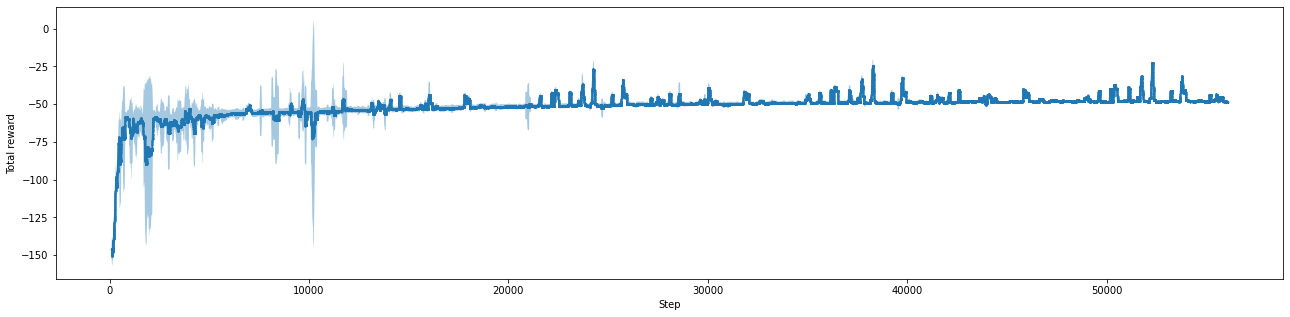
\includegraphics[width=.8\linewidth]{images/MVOberr/RL/RLrewards.png}
    \caption[Agent's rewards]{Agent's rewards over time. The reward is averaged over a rolling window of 96 time steps. The shadow region is $\pm2$ standard deviations calculated over 5 runs.}
    \label{im:4_rewards}
\end{figure}
\noindent From figure \ref{im:4_rewards}, it is possible to see that the agent is learning, since the total reward is increasing over time.\\

For all the 5 runs, after training, the agent was evaluated on the test set. Here reported are the results from one of the best run:
\begin{figure}[h]
\centering
    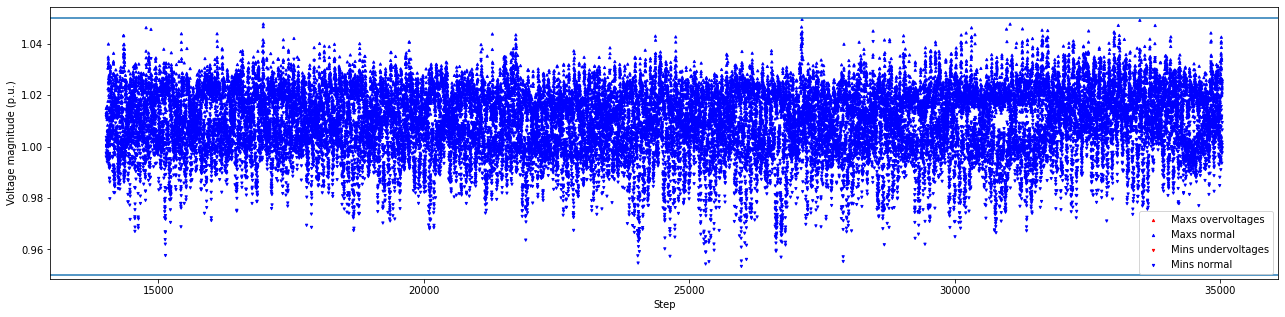
\includegraphics[width=0.9\linewidth]{images/MVOberr/RL/CritialSituationsAfter.png}
    \caption[Agent's solution to voltage problems]{The buses' voltage situation after the agent's actions.}
    \label{im:4_prosolv}
\end{figure}
\noindent Figure \ref{im:4_prosolv} shows that the agent was able to solve all the over voltage problems without introducing under voltages problems, that were solved as well.

\begin{algorithm}[h]
    \STATE Total energy 169187 MW, total curtailed energy: 0.91 MW in 21024 time steps (7 months and 13 days), ratio: $5.3 \cdot 10^{-6}$ \%\\
    
    \STATE Total reactive power controlled: 287085 M\gls{VAR}
\end{algorithm}
\noindent the percentage of curtailed energy is well below the tolerable values of 4\%. Indeed, curtailment levels have generally been 4\% or less of wind energy generation in regions where curtailment has occurred.\\
While the reactive power corresponds to an average of 0.22 M\gls{VAR} for device.\\

\noindent Some statistic from figure \ref{im:4_prosolv} are  reported here:

\begin{algorithm}[h]
    \STATE Maximum voltage observed: 1.0494 p.u. \\
    \STATE Minimum voltage observed: 0.9533 p.u.
\end{algorithm}
\noindent So the agent understood how to control the network minimising the control needed, since the values are really close to the boundaries (1.05 p.u. and 0.95 p.u.) but inside the safe voltage condition.\\

In all the 5 runs the agent was able to solve the over voltage problems and in only one run some under voltages conditions were not solved.\\
It has also must be said that the agent performance is not perfect since the agent took some actions even it was not needed, it is also possible to see from figure \ref{im:4_rewards} is stuck in a local minimum, since the reward is steady around $-50$. \\

\noindent Here there are some more statistics for the best run:\\

\begin{algorithm}[h]
    \STATE Active power curtailment:\\
    \STATE needed (case 3: 1 - 0): 0.67 MW\\
    \STATE Not needed:\\
    \STATE case 1 (0 - 0): 0.24 MW\\
    \STATE case 2 (0 - 1): 0 MW\\
    \STATE case 4 (1 - 1): 0 MW\\
    
    \STATE Reactive power usage:\\
    \STATE needed (case 3: 1 - 0): 106341 MVAR\\
    \STATE Not needed:\\
    \STATE case 1 (0 - 0): 180744 MVAR\\
    \STATE case 2 (0 - 1): 0 MVAR\\
    \STATE case 4 (1 - 1): 0 MVAR
\label{alg:agentsucks}
\end{algorithm}
\noindent Cases, as defined in \ref{im:cases}, are reported here to check in which situation the agent decides to take a particular action.\\
In particular, the agent is able to understand when it is needed to perform the action (case 3) and in all those cases it can solve the voltage critical situation (case 4 situations are 0). Moreover, the agent newer worsened the situation of the network (case 2 situations are 0) but the agent could perform better since a lot of activity is done when not really needed (case 1).


\section{Conclusions and further works}
This master's thesis has investigated the analysis and the use of machine learning techniques to forecast some possible over voltage problems in a power network and to carry out some possible active control of its devices to reduce the number of critical situations.\\

In particular, for the forecasting part, results showed that it is possible to forecast the network's critical situation, in particular the most performing model is the recurrent neural network with 30 minutes of past buses' voltage information, obtaining an accuracy of 0.981 and a F1-score of 0.826.\\
Some techniques for unbalanced databased were used as well, improving the score of the least performant model and keeping them unchanged for the best performant one.\\

For the control part, a reinforcement leaning training method was used to train an agent to avoid over voltages problems. The model used was a deep deterministic policy gradient algorithm. This algorithm was able, using only  15 minutes of the network's information, to solve the critical situations in the network. In particular, the agent was able to solve 100\% of the over voltage problems and, most of the time, 100\% of the under voltage problems as well; with a cost for the distribution system operator of few MWs of active power in the entire time span considered of 7 months and 13 days.